\newcommand{\figureLCDCharAnimation}[1]{
  \def\lang{\detokenize{#1}}
  \def\langRu{\detokenize{ru}}
  \def\langEn{\detokenize{en}}
  \def\figureCaption{XXX: No translation.}
  \ifx \lang\langRu
  \def\figureCaption{
    Три варианта изображение игрока: смотрящий влево (``LEFT''), бездействующий
    (``IDLE'') и смотрящий вправо (``RIGHT''.)
  }
  \fi
  \ifx \lang\langEn
  \def\figureCaption{
    Three variants of the player image: looking left (``LEFT''), idle (``IDLE'')
    and looking right (``RIGHT''.)
  }
  \fi
  \begin{figure}[ht]
    \centering
    \def \offsetLeft{0.0}
    \def \offsetIdle{3.5}
    \def \offsetRight{7.0}
    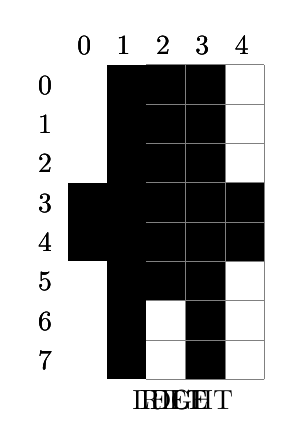
\begin{tikzpicture}
      %% Left.
      %% 0
      \fill[black] (\offsetLeft + 0.5, 0) rectangle (\offsetLeft + 2.0, -0.5);
      %% 1
      \fill[black] (\offsetLeft + 1.0, -0.5) rectangle (\offsetLeft + 2.0, -1.0);
      %% 2
      \fill[black] (\offsetLeft + 1.5, -1.0) rectangle (\offsetLeft + 2.0, -1.5);
      %% 3
      \fill[black] (\offsetLeft + 0.0, -1.5) rectangle (\offsetLeft + 2.0, -2.0);
      %% 4
      \fill[black] (\offsetLeft + 1.5, -2.0) rectangle (\offsetLeft + 2.0, -2.5);
      %% 5
      \fill[black] (\offsetLeft + 1.0, -2.5) rectangle (\offsetLeft + 2.0, -3.0);
      %% 6
      \fill[black] (\offsetLeft + 2.0, -3.0) rectangle (\offsetLeft + 1.5, -3.5);
      \fill[black] (\offsetLeft + 1.0, -3.0) rectangle (\offsetLeft + 0.5, -3.5);
      %% 7
      \fill[black] (\offsetLeft + 2.0, -3.5) rectangle (\offsetLeft + 1.5, -4.0);
      \fill[black] (\offsetLeft + 1.0, -3.5) rectangle (\offsetLeft + 0.5, -4.0);
      \draw[step=0.5cm,gray,very thin] (\offsetLeft, -4.0) grid (\offsetLeft + 2.5, 0);
      %% Numbers
      \foreach[count=\n from 0] \x in {0.0, 0.5, ..., 2.0} {
        \draw (\offsetLeft + \x cm, 0 cm) node[anchor=south west] {$\n$};
      }
      \foreach[count=\n from 0] \y in {-0.5, -1.0, ..., -4.0} {
        \draw (\offsetLeft - 0.5 cm, \y cm) node[anchor=south west] {$\n$};
      }
      \draw (\offsetLeft + 0.7, -4.5) node[anchor=south west] {LEFT};

      %% Idle.
      %% 0
      \fill[black] (\offsetIdle + 2.0, 0) rectangle (\offsetIdle + 0.5, -1.0);
      %% 2
      \fill[black] (\offsetIdle + 1.0, -1.0) rectangle (\offsetIdle + 1.5, -1.5);
      %% 3
      \fill[black] (\offsetIdle + 0.5, -1.5) rectangle (\offsetIdle + 2.0, -2.0);
      %% 4
      \fill[black] (\offsetIdle + 2.0, -2.0) rectangle (\offsetIdle + 2.5, -2.5);
      \fill[black] (\offsetIdle + 1.5, -2.0) rectangle (\offsetIdle + 1.0, -2.5);
      \fill[black] (\offsetIdle + 0.5, -2.0) rectangle (\offsetIdle + 0.0, -2.5);
      %% 5
      \fill[black] (\offsetIdle + 0.5, -2.5) rectangle (\offsetIdle + 2.0, -3.0);
      %% 6
      \fill[black] (\offsetIdle + 2.0, -3.0) rectangle (\offsetIdle + 1.5, -3.5);
      \fill[black] (\offsetIdle + 1.0, -3.0) rectangle (\offsetIdle + 0.5, -3.5);
      %% 7
      \fill[black] (\offsetIdle + 2.0, -3.5) rectangle (\offsetIdle + 1.5, -4.0);
      \fill[black] (\offsetIdle + 1.0, -3.5) rectangle (\offsetIdle + 0.5, -4.0);
      \draw[step=0.5cm,gray,very thin] (\offsetIdle, -4.0) grid (\offsetIdle + 2.5, 0);
      %% Numbers
      \foreach[count=\n from 0] \x in {0.0, 0.5, ..., 2.0} {
        \draw (\offsetIdle + \x, 0) node[anchor=south west] {$\n$};
      }
      \foreach[count=\n from 0] \y in {-0.5, -1.0, ..., -4.0} {
        \draw (\offsetIdle - 0.5, \y ) node[anchor=south west] {$\n$};
      }
      \draw (\offsetIdle + 0.8, -4.5) node[anchor=south west] {IDLE};

      %% Right.
      %% 0
      \fill[black] (\offsetRight + 0.5, 0) rectangle (\offsetRight + 2.0, -0.5);
      %% 1
      \fill[black] (\offsetRight + 0.5, 0) rectangle (\offsetRight + 1.5, -1.0);
      %% 2
      \fill[black] (\offsetRight + 0.5, -1.0) rectangle (\offsetRight + 1.0, -1.5);
      %% 3
      \fill[black] (\offsetRight + 0.5, -1.5) rectangle (\offsetRight + 2.5, -2.0);
      %% 4
      \fill[black] (\offsetRight + 0.5, -2.0) rectangle (\offsetRight + 1.0, -2.5);
      %% 5
      \fill[black] (\offsetRight + 0.5, -2.5) rectangle (\offsetRight + 1.5, -3.0);
      %% 6
      \fill[black] (\offsetRight + 2.0, -3.0) rectangle (\offsetRight + 1.5, -3.5);
      \fill[black] (\offsetRight + 1.0, -3.0) rectangle (\offsetRight + 0.5, -3.5);
      %% 7
      \fill[black] (\offsetRight + 2.0, -3.5) rectangle (\offsetRight + 1.5, -4.0);
      \fill[black] (\offsetRight + 1.0, -3.5) rectangle (\offsetRight + 0.5, -4.0);
      \draw[step=0.5cm,gray,very thin] (\offsetRight, -4.0) grid (\offsetRight + 2.5, 0);
      %% Numbers
      \foreach[count=\n from 0] \x in {0.0, 0.5, ..., 2.0} {
        \draw (\offsetRight + \x, 0) node[anchor=south west] {$\n$};
      }
      \foreach[count=\n from 0] \y in {-0.5, -1.0, ..., -4.0} {
        \draw (\offsetRight - 0.5, \y) node[anchor=south west] {$\n$};
      }
      \draw (\offsetRight + 0.8, -4.5) node[anchor=south west] {RIGHT};
    \end{tikzpicture}
    \caption{\figureCaption}
    \label{fig:game-dev-player-textures}
  \end{figure}
}
